\chapter{Network Models}\label{network_models}


%% Collectors Profiling and activities history
%%%% Profiling collectors in terms of their activities and interests can be a way of further detecting anomalies (activity monitoring, Fawcett and Provost 1999).





In this chapter we present and formally describe two classes of network models that were developed during this study.
\textbf{Species-collectors networks} (SCNs) are built based on associations between collectors and the species they've recorded during their careers, whereas \textbf{collectors coworking networks} (CWNs) describe direct collaborative associations between collectors when recording specimens in field.

Although structurally distinct, models here presented provide complementary perspectives on the recording behavior of collectors from a given species occurrence dataset. 
From SCNs we retrieve information on which collectors have recorded which species and, conversely, which species were recorded by which collectors. 
CWNs, on the other hand, allow us to investigate which collectors team up with whom during fieldwork, although here species are not represented as entities.

As both models were elaborated based on a social networks analytics framework, we start by reviewing some general concepts from the network science domain.

% What am I modeling with these models?

\section{Complex Networks: A theoretical background}
\subsection{The rise of the study of complex networks}
%% The rise of the field of complex networks
%% A historical background
%% Applications (biology and other fields)
%% What are complex networks?
%%%% Random networks, small-world and scale-free topologies 

\subsection{Mathematical Representations}
% Networks are mathematically represented as graphs
%% Nodes and Edges
%%% Edges are established between a pair of nodes , recurrent edges
%%% Nodes and edges can have attributes (each attribute holding values)
%%% Neighborhood, neighbors
%%% Cliques
%%% Paths 

Networks are mathematically represented as graphs.

\paragraph*{Graphs}
Graphs are formally defined as a 2-tuple $G=(S,E)$ containing a set of nodes $S$ and a set of edges $E$.

\paragraph*{Connected components}
For undirected graphs, connected components are defined as subgraphs in which there is at least one path linking each pair of nodes.

%% Graph density
%%% Fully connected: n*(n-1)/2


%% Matrix Representation
%%% Adjacency matrix, sparsity
For some applications it turns to be convenient to use a matrix representation of graphs. A matrix where ... is known as the graph's \textbf{adjacency matrix}. % where are zeros and ones?
In case the graph is unimodal the adjacency matrix is a squared symmetrical matrix.
For bipartite graphs, however, this is not necessarily true. It depends on the size of each nodes set. We refer to it as the \textbf{biadjacency matrix}.

%% Degree
%%%% Degree distribution
%%%% Power laws
%%%%% Many real-world networks are approximately scale-free (give examples)
%%%% Machanism: Preferential attachment, rich gets richer: Higher degree nodes (richer), lower degree nodes (poorer)

\subsection{Bipartite Graphs}
%% Bipartite graphs
%%%% The bipartite constraint: formalization: Nodes sets are DISJOINT (no intersection) ; and INDEPENDENT (no adjacent nodes within any set); 
%%%% Biadjacency matrix
%%%% Bipartite projection
%%%%%% bipartite tradeoff : summarization vs information loss
%%%%%% bipartite projections edges set is usually very dense -> The importance of adding weights to edges in bipartite projections
%%%%%% weaker connections are then filtered out

  \begin{figure}[h!]
  	\centering
    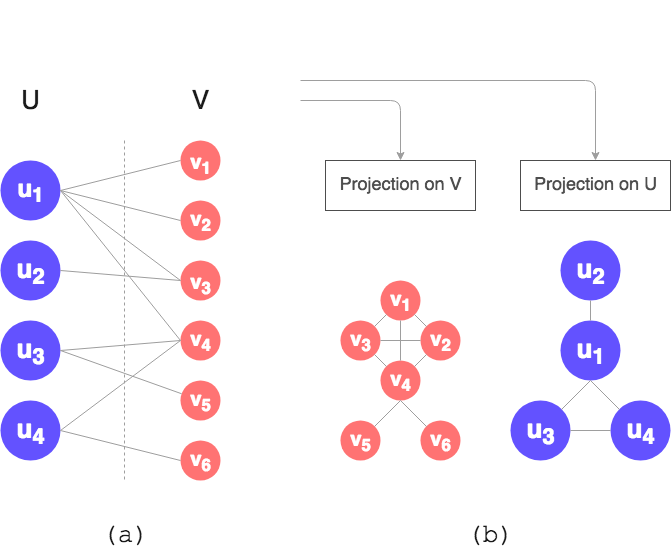
\includegraphics[width=0.5\linewidth]{figures/bipartite_general.png}
    \caption{(a) General aspect of a bipartite graph. All nodes in the graph belong to exactly one of $U$ and $V$ nodes sets. In addition edges are only established between nodes from distinct sets. (b) Bipartite projections. Projections onto each node set are constructed by linking together nodes that are at a length-2 distance in the bipartite graph, while omitting nodes from the other set.}
    \label{fig:bipartite_general}
  \end{figure}






% ===========================
% ===========================
% Species-collectors Networks
% ---------------------------
%% TODO: SCNs do not allow 0-degree nodes

\section{Species-collectors Networks}

In this section we describe Species-collectors Networks (SCNs) as a relational model for structuring associations between collectors and species.
We first give an overview on the semantics of the relationships we propose to model and how they can be derived from a species occurrence dataset.
Next we define attributes and operations for SCNs that facilitate obtaining domain-specific insights from it.
Finally we compare our proposed model to other analogous though different systems in literature.


\subsection{General Description}

%% Model semantics
Species-collectors networks describe relationships of type ``\textbf{collector} samples \textbf{species}'' or, conversely, ``\textbf{species} is sampled by \textbf{collector}''. Such relationships, which necessarily involve both a collector and a species, are structured as links in the network.
The network is thus composed by collectors holding links to every single species she has ever recorded or alternatively, species holding links to every collector who have ever recorded them.
An important semantic aspect of this model worth emphasizing is that here we model collectors recording species rather than specimens. As exposed elsewhere in this text, the term ``species'' refers to aggregations of taxonomically similar \textit{specimens}, which are the actual individuals that are collected. Thus, while collectors are represented at the individual level (each collector is a person), species are instead entities composed of groups of individuals, and must be uniquely included in the network as such.
This means no particular collector or species should be represented more than once in the model, even though they might have been observed in multiple records in dataset.

%% Model specification
As networks are formally described as graph structures, we represent both collectors and species entities as nodes, though belonging to distinct classes.
Links are represented as edges.
Moreover, as relationships here modeled can only possibly exist between collectors and species we also impose a constraint that all edges in the work must necessarily connect nodes from distinct classes. In other words, nodes can be divided into two disjoint sets, with the condition that no edges in the same set are adjacent.
This best matches the description of a bipartite network
$$ SCN = (S_{col},S_{sp},E) \mbox{ ,}$$
where $S_{col} = \{u_1, u_2, ..., u_n \}$ is the nodes set representing the collectors group; $S_{sp}=\{v_1,v_2, ..., v_m\}$ is the nodes set representing the species group; and $E$ is the set of undirected edges between members of $S_{col}$ and $S_{sp}$.

The graph can also be represented as a rectangular biadjacency matrix $A^{n\times m}$ for which $a_{ij}\neq 0$ \textit{iff} $(u_i,v_j) \in E$. Values of non-zero $a_{ij}$ elements are set to the number of times edges $(u_i,v_j)$ occur in the network, as described below. 
For large and sparse SCNs, storage and operations on the graph object can be optimized by using sparse matrix designs for $A$.

  \begin{figure}[h!]
  	\centering
    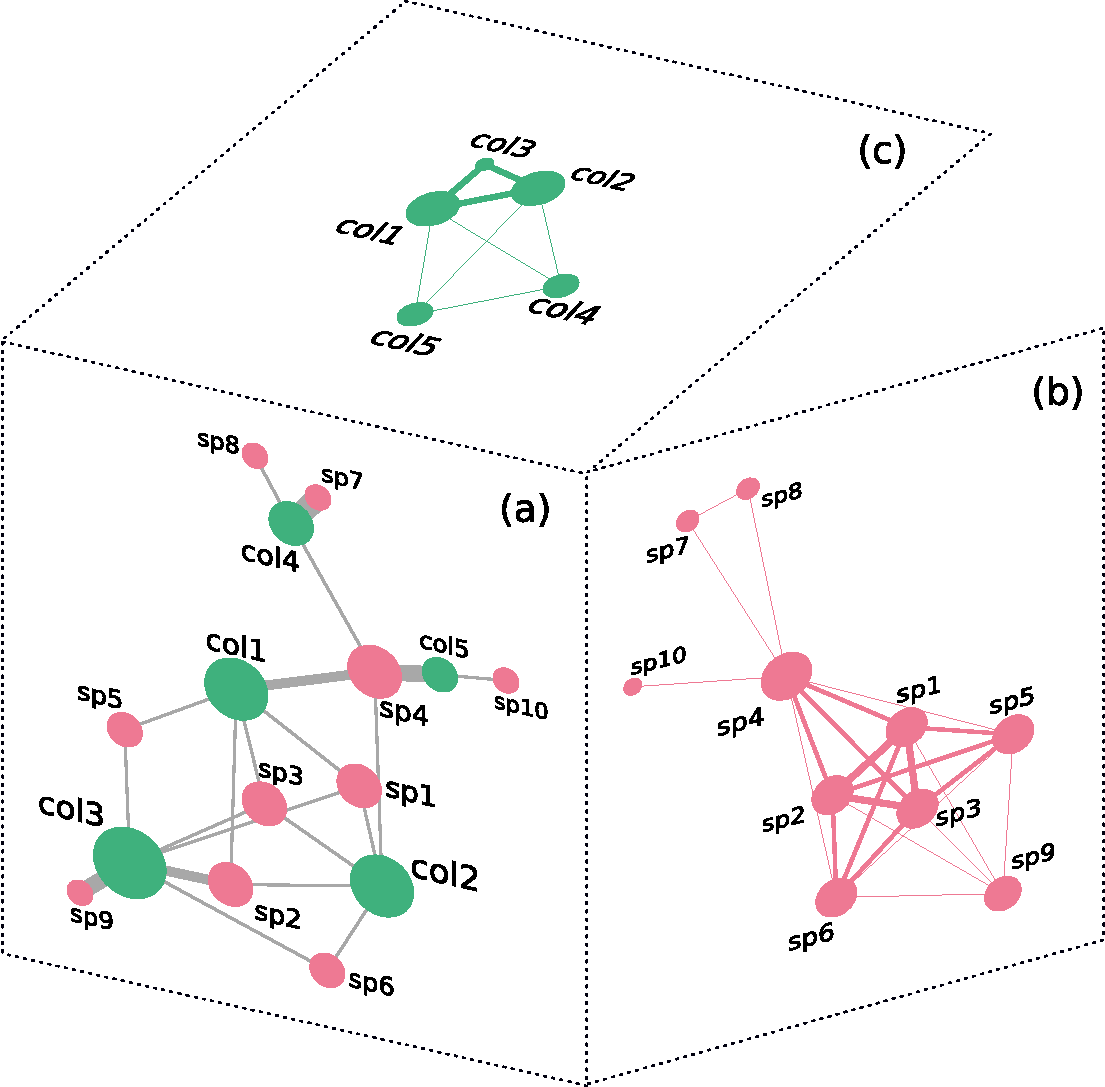
\includegraphics[width=.7\linewidth]{figures/network_models/scn_generalaspect.pdf}
    \caption{Multiple perspectives of a species-collectors network model (SCN).
    (a) Unprojected network, where collectors (green nodes) are linked to the species (red nodes) they've recorded. The total number of records of a given species by some collector is reflected in the strength of their link. (b) SCN projection onto the species set. Species are linked together if they've been collected by common collectors. Link strength is proportional to the number of collectors two species share. (c) SCN projection onto the collectors set. Collectors are linked together if they've recorded species in common. Link strength is proportional to the number of species two collectors share. 
    Link strength for both projections were obtained using the \textit{simple weighting} rule, and are graphically displayed as edges thickness.}
    \label{fig:scn_general}
  \end{figure}
  
%% Network construction
\subsection{Model construction from data}
% the construction process, using paired collectors-species lists guarantees that no disconnected node can possibly exist
We use basically two fields to build a SCN model from a species occurrence dataset. First, we need a collectors field, containing the names of all collectors that were responsible for the record; and the species field, storing the name of the species if determined up to that taxonomic resolution.
Following Darwin Core terms standard\footnote{\url{http://rs.tdwg.org/dwc/terms/}}, we should expect to find collectors names in the \textit{recordedBy} field; and the species name in a field named \textit{species}. As not every biological collection dataset uses Darwin Core standards though, these fields might be occasionally found under different names.

The network is built up from the dataset in an iterative process. For each row in the dataset each individual collector included in the record establishes an additional link to the collected species.
In this process nodes and edges are either created in case they did not previously exist in the graph; or have their occurrence counts increased in case they did.
We keep the record of the number of times each link occurs in the network by setting a \textit{count} attribute to them, which is initially set to $1$ and is increased by one every time a new occurrence of the link is observed. Link strength is proportional to this attribute, and is graphically represented by edges thickness (Figure \ref{fig:scn_general}).
The more often a particular collector records a particular species, the stronger gets the link between them.
An homonymous attribute is also set to graph nodes, which is increased whenever a new link involving the node is either added or strengthened. As a result the node's \textit{count} attribute keeps a record of how many times a given species or collector occurs in the dataset.
The reader should note, however, that \textit{count} attributes for nodes and edges are conceptually distinct and are not to be confused.

Edges' \textit{count} values are stored in the biadjacency matrix $A$, and thus the value of element $a_{ij}$ is the number of times the edge $(u_i, v_j)$ occurs. An example of a SCN network is given in Figure \ref{fig:scn_general}, for which the adjacency matrix is
$$
A =
\kbordermatrix{
& sp1 & sp2 & sp3 & sp4 & sp5 & sp6 & sp7 & sp8 & sp9 & sp10 \\
col1 & 1 & 1 & 1 & 2 & 1 & 0 & 0 & 0 & 0 & 0 \\
col2 & 1 & 1 & 1 & 1 & 0 & 1 & 0 & 0 & 0 & 0 \\
col3 & 1 & 2 & 1 & 0 & 1 & 1 & 0 & 0 & 3 & 0 \\
col4 & 0 & 0 & 0 & 1 & 0 & 0 & 4 & 1 & 0 & 0 \\
col5 & 0 & 0 & 0 & 3 & 0 & 0 & 0 & 0 & 0 & 1 \\
}.
$$

% ===============
% SCN Definitions

\subsection{Definitions}
Attributes and operations for retrieving information about species and collectors.
Operation for summarizing the model.
In this section I define some attributes of the SCN model 

\paragraph{Species bag.} 
The entire set and counts of species a collector has recorded in a dataset, which can be thought as a collector's species signature, composes his/her \textit{species bag}. This attribute is therefore exclusively derivable for collectors nodes.
As species bags are directly obtained as row-vectors of the graph's biadjacency matrix, they are a convenient structure for comparing collectors in terms of the composition of their records.
For that task a high variety of well-known distance algorithms for vectors in literature can be readily applied.
The species bag $\sigma$ for collector $u_i$ is defined as

$$
\sigma_{u_i} =  \begin{bmatrix}
a_{i 1}, a_{i 2}, ..., a_{i m}
\end{bmatrix}  \quad ,
$$
where $m$ is the length of the species set and each $a_{i j}$ is the total number of records of species $v_j$ by collector $u_i$. The sum of all elements in a collector's species bag, which is equivalent to the vector's \textit{l1 norm} $||\sigma_{u_i}||_1$, corresponds to the total number of records for that collector.

 
\paragraph{Quorum.} 
The entire set and counts of collectors who have recorded a particular species in a dataset comprise its \textit{quorum}, an exclusive attribute of species nodes. 
This concept can be thought as the inverse of a species bag, being the collectors signature of a species. 
The quorum vector $\iota$ of a species $v_j$ is directly obtained from the graph's biadjacency matrix as the $j^{th}$ column-vector 

$$
\iota_{v_j} = \begin{bmatrix}
a_{1 j}, a_{2 j}, ..., a_{n j}
\end{bmatrix} \quad ,
$$
where $n$ is the length of the collectors set and each $a_{i j}$ is the total number of times collector $u_i$ has recorded species $v_j$. 
The total number of occurrences of species $v_j$ in the entire dataset can be obtained as the sum of all elements in its quorum vector $ || \iota_{v_j} ||_1$.


\paragraph{Taxonomic aggregation and resolution.}
In some contexts it might be desired to simplify SCNs by grouping species nodes into higher taxonomic ranks (or levels), such as \textit{genus} or \textit{family}. This process is defined as \textit{taxonomic aggregation}, and is performed by 
($i$) obtaining a grouping of species using some taxonomic rank; 
($ii$) obtaining quorum vectors for each species; 
($iii$) summing up quorum vectors for all species in each group;
($iv$) building a new SCN model, aggregated on rank T. 
The SCN's \textit{taxonomic resolution} is the taxonomic rank at which species are aggregated in the model. For the sake of model interpretability, all nodes in $S_{sp}$ must necessarily be represented as taxons belonging to the same rank as the SCN's taxonomic resolution.

For a more formal description let $G_T = \{g_1,g_2,..., g_n\}$ denote a taxonomic grouping at rank $T$, containing a set of $n$ rank-$T$ taxa.  In addition, let each taxon $g_i \in G_T$ itself be a set of nodes $S_{sp}^{(i)} \subseteq S_{sp}$, with the conditions that there are no empty $S_{sp}^{(i)}$ and that every node $v \in S_{sp}$ is a member of exactly one set  from $ \{ S_{sp}^{(1)}, S_{sp}^{(2)}, ..., S_{sp}^{(n)} \}$.
Such a grouping rule makes $G_T$ a partition of $S_{sp}$, and thus the entire set $S_{sp}$ can be recreated by simply computing the union of elements in $G_T$. This guarantees that no entities are duplicated or eliminated on aggregations using it.

We then use grouping $G_T$ for obtaining quorum vectors for each of its taxa $g_i \in G_T$, which will be represented as nodes in the new aggregated graph. Quorum vectors are computed as $ \iota_{g_i} := \sum_j \iota_{v_j}  $ for $v_j \in S_{sp}^{(i)}$. Finally, the rank-$T$ aggregated  graph $SCN_T=(G_T,S_{col},E)$ is created from a biadjacency matrix, which is constructed by stacking quorum vectors for each taxon $g_i$ as row-vectors. The set of collectors nodes remain the same in the aggregated graph.

% The PICI model (Lambiotte2005)
%% Collective effects acting on individuals with similar interests
%% Individual mechanisms, pushing collectors towards their particular interests, establishing their collecting niche

% Temporal edges


% ===============
% SCN projections
\subsection{Projections}

Bipartite projections on each one of the SCN's nodes sets allows one to investigate indirect associations two entities from the same class might have with each another, as intermediated by a third entity from the opposite class. 
Figure \ref{fig:scn_general} illustrates projections of a SCN onto the species set (b) and the collectors set (c).
In overall, each projection gives us complementary perspectives of transitive relationships in the SCN, either from the collectors or species point of view.

From a species-centric perspective (Figure \ref{fig:scn_general}b), connections are formed between species having been recorded by at least one collector in common, with link strength proportional to the number of different collectors they share. 
Although collectors are used during projection for determining the existence of links between species they are not represented as nodes in this projection.
In general strongly connected species can be interpreted as being both included in the species bags of many collectors, whereas weakly connected or isolated species are seldom or never recorded by the same collectors.
% Modules in species projections reveal species that are more intensely associated with each other than with others from outside the module
The second perspective (Figure \ref{fig:scn_general}c) is collectors-centric, in that only collectors are represented as nodes whilst species are omitted. 
Analogously to the species-centric perspective, here collectors are linked together if they have recorded at least on species in common, with link strength depending on the number of shared species between them. 
From this perspective we could identify collectors having similar recording profiles.

As previously discussed in this text, projections are a mechanism for summarizing bipartite into more convenient one-mode graphs, where only one class of entity is represented. % TODO: Remember to add this in the projection section
Projections, however, come with the cost of information loss, as any relationships or attributes of nodes from the omitted set are not represented in the projection \cite{Borgatti1997}. % TODO: Add reference
Moreover, relevant associations between entities eventually become obfuscated by others of lower relevance, as projections tend to generate graphs that are much denser than the original bipartite model \cite{Lambiotte2005}.
Choosing an appropriate weighting rule for the aspects one wants to investigate is thus detrimental for separating relevant from less-relevant associations, so that the latter ones can be subsequently removed by applying weighting filters.
Below I first describe the simplest weighting rule with its limitations and, in sequence, some alternatives rules for overcoming them.
% https://doi.org/10.1016/j.physa.2006.12.021 <- The effect of weight on community structure of networks

\paragraph*{Simple weighting.}
This rule assigns weights to links between pairs of collectors ($u_s$ and $u_t$) or species ($v_s$ and $v_t$) by simply counting the total number of species collectors share on their species bags or the total number of collectors species share in their quorum vector. The rule is mathematically expressed as:
\begin{equation} \label{eq:simple_weighting}
\begin{split}
w_{(u_s, u_t)} &= \sum_{j=1}^{m} \delta(\sigma^{(j)}_{u_s}, \sigma^{(j)}_{u_t})\mbox{ , for the projection onto }S_{col}\mbox{ ;}\\
w_{(v_s, v_t)} &= \sum_{i=1}^{n} \delta(\iota^{(i)}_{v_s}, \iota^{(i)}_{v_t})
\mbox{ , for the projection onto }S_{sp}\mbox{, where}
\end{split}
\end{equation}
$n = |S_{col}|$, $m = |S_{sp}|$, $\sigma^{(i)}$ and $\iota^{(i)}$ are the $i^{th}$ element of a species bag and a quorum vector, respectively; and $\delta(u,v)=1$ if both $u$ and $v$ are non-zero and $0$ otherwise.

In order to obtain the weights for every pairs of projected nodes more efficiently we can use a vectorized implementation of this rule. First we derive a $n\times m$ logic matrix $A_{bool}$ from the SCN biadjacency matrix $A$ by simply replacing its non-zero elements by ones. 
Then a $n \times n$ adjacency matrix with edges weights for the $S_{col}$ projection is obtained by calculating the dot product $A_{bool} A_{bool}^T$.
Conversely, for the $S_{sp}$ projection, the $m \times m$ weights matrix is obtained by calculating $A_{bool}^T A_{bool}$.

The simple weighting rule has an important limitation when applied to SCNs.
It arises from the fact that the weight assigned to edges linking pairs of nodes in the projection only reflects the number of distinct intermediate neighbors from the complementary set they shared in the non-projected graph. The number of times each species is recorded by each collector is therefore ignored while computing the strength of links in the projections, underestimating the importance of recurrent relationships.
Consequently this weighting rule tends to make very prolific and generalist collectors or very attractive species strongly connected to many others in a disproportional way, as an effect of their high degrees in the non-projected model. The opposite happens in the case of specialized nodes, which typically hold fewer --- although recurrent --- distinct links to their neighbors. 
In order to reduce these effects two alternative rules are proposed below.

\paragraph*{Additive weighting.}
This rule is a slight modification of the simple weighting rule, in that it also considers the total number of times entities interact through each neighbor-intermediated path in the non-projected network. The rule is expressed using the same equations from (\ref{eq:simple_weighting}), but changing the $\delta$ function to
 
$$\delta(u,v) = 
\begin{cases}
\frac{u+v}{2} &  \mbox{if both } u \mbox{ and } v \mbox{ are non-zero ,}\\
0 & \mbox{otherwise}
\end{cases}
$$
In case every distinct path in the non-projected SCN only occur once then both simple and additive weighting rules lead to the same result. % TODO: Test this assumption 
This modified rule potentializes the effect of recurring edges from the non-projected graph on computing edges weights in the projection, thus reducing weighting asymetries from generalist and specialized nodes.

However, this approach still has a drawback in that nodes which have high degrees in the non-projected graph tend to become much more strongly connected with themselves in the projection than average-degree ones, simply by the fact that they have many more connections than average.
Additionally, without a superior limit for the $\delta$ function it turns out to be hard to determine a proper threshold when filtering relevant from non-relevant edges. The next weighting rule is designed to reduce the effects of nodes degrees on their edges' weights, outputting values which are bounded to the $[0,1]$ interval.

\paragraph*{Species bag / Quorum similarity.}
% This is called "Structural Equivalence": Nodes have ties to common third-parties {Borgatti2015}
% One characteristic is that in practice collectors holding similarity values very close to one tend to be those with very few records in the dataset. More experienced collectors can have higher similarities with some collectors, but it is usually not very high.
This weighting rule uses a similarity (or correlation) matrix that is computed for each projection of the SCN. Edges' weights are given by the similarity between their nodes. The similarity matrix for the collectors and species projections are constructed by computing the  \textit{cosine similarity} of species bags and quorum vectors  for each pair of nodes in the respective projection. 
The \textit{species bag similarity} for collectors $u_s$ and $u_t$ and the \textit{quorum vector similarity} for species $v_s$ and $v_t$ are defined as

\begin{equation}
\begin{split}
sim(\sigma_{u_s},\sigma_{u_t}) &\equiv
\cos \theta_{u_s,u_t} =
\frac{  \sigma_{u_s} \cdot \sigma_{u_t}  }{  ||\sigma_{u_s}||_2  ||\sigma_{u_t}||_2  } \\
sim(\iota_{v_s},\iota_{v_t}) &\equiv
\cos \theta_{v_s,v_t} =
\frac{  \iota_{v_s} \cdot \iota_{v_t}  }{  ||\iota_{v_s}||_2  ||\iota_{v_t}||_2  } 
\end{split}
\end{equation}

Therefore each element in the similarity matrix holds the edge weight for a pair of nodes, with a value ranging within the interval $[0,1]$. Edges weights are zero-valued if no direct link exist between two nodes,  whilst nodes linked by edges with a weight of $1$ have identical species bags or quorum vectors. Intermediate values reflect the correlation measure obtained for node pairs.
As this rule outputs weight values that are bound to a known interval, filtering less relevant links become much more straightforward. Depending on the aspects regarding the species-collectors system an investigator might be interested in, a filtering threshold $\phi$ can be set based on the minimum correlation value she considers acceptable, such that only the most relevant relationships for that particular analysis are kept.
%%% check neighborhood similarity functions in literature
%% Edges pruning


\subsection{Conclusion}
Whereas SCNs represent ..., other structures might arise when analyzing which collectors record together. 
The model presented in the next section covers this.










% =============================
% =============================
% Collectors Coworking Networks
% -----------------------------

\section{Collectors Coworking Networks}
% References: (Ramasco2004)

% TODO: update: CWNs do allow nodes with 0 degree (collectors who have never collaborated)
Collectors coworking networks (CWNs) describe coauthoring relationships between collectors. Two collectors are considered to be co-authors in a particular record if they are both included as collectors responsible for that occurrence. In other words, these models represent collectors who have worked together in field, having recorded specimens collaboratively.
In a dataset following \textit{Darwin Core} standards collectors names are obtained from the $recordedBy$ field.
A CWN is constructed from an occurrences dataset by iterating over each record and forming \textit{clique} structures with the associated collectors, which are finally combined into a single undirected graph formally represented as 
$$CWN = (S,E) \mbox{ ,}$$
where $S$ and $E$ are the graph's nodes and edges sets representing, respectively, collectors and links connecting them. This construction process is illustrated in Figure <>. % create figure %

As opposed to SCNs, CWNs model collaborative relationships between entities of the same type, thus all nodes in the graph belong to the same class and are contained in the nodes set $S$. 
Although species are not represented as entities in this model, a vector with all taxa recorded collaboratively by two collectors is included as an attribute of the edge connecting them, in addition to its \textit{count} attribute.
Edges linking each pair of collectors are unique in the graph, and the total number of times that association occurs in the dataset is included as an attribute of the edge.

% Are unconnected collector represented in the model?

Weights can be assigned to edges in the CWN as a measure of their overall relevance in the network structure. Edges with higher weight values represent stronger collaborative ties between collectors, pointing out the main groups of collectors who are most willing to collaborate. 
The simplest rule is to set the edge weight as its total total number of occurrences. However, as pointed out by other authors studying social networks \cite{Newman2001a}, in reality not all collaborations contribute the same way for a collector's network. 
Collectors tend to hold weaker collaborative ties with each other when they collaborate in larger teams than when they collaborate in smaller ones. The hyperbolic weighting rule, described below, accounts for this fact, while also considering the total number of collaborations between two collectors as a factor contributing the strength of their link.

\paragraph*{Hyperbolic weighting.}
If we wanted to set edges weights to the same value as the total counts of their occurrences, we would simply increase the weight value by one for each new occurrence of a given link, during the construction of the network model. 
If we use the hyperbolic weighting rule instead not every new occurrence of the link increases the edge weight by one. 
The contribution of each new link depends on the number of the collectors $n^{(k)}$ included in record $k$ or, in other words, its clique size. 
This rule follows a hyperbolic growth function 
\begin{equation}
w_{(i,j)} = \sum\limits_k \frac{\delta_i^{(k)} \delta_j^{(k)}}{(n^{(k)}-1)} \mbox{ , }
\end{equation}
where $\delta^{(k)}_u = 1$ if collector $u$ is in record $k$ and $0$ otherwise.
As the hyperbolic function above has singularity at $1$, it gets ill-defined for records with only one collector. 
Therefore only records with two or more collectors are used to compute edges weights. 
The maximum weight contribution of 1 is assigned to records with two collectors, whilst records with larger cliques yield smaller contributions.\\


% Weighting rules



% Basic node attributes
The degree ($k$) for a node depends on the total number of edges it holds. 
This metric informs us how many different other collectors a collector has ever collaborated with.
In case we also want to consider the effect of the weights associated to each edge in the degree metric we must compute the weighted degree ($k_w$).
The \textbf{strength} of a node is the sum of the weights associated to all its edges. It describes the total number of collaborative records for a collector.
%% Average number of collaborators?


%% Weighting
%%% Check the weighting rule from Newman2001a -> Hyperbolic weighting